% !TeX root = template.tex
%!BIB program = bibtex
%%%%%%%%%%%%%%%%%%%%%%% file template.tex %%%%%%%%%%%%%%%%%%%%%%%%%
%
% This is a template file for the LaTeX package SVJour2 for the
% Springer journal "Machine Vision and Applications".
%
%                                    Springer Heidelberg 2004/11/04
%
% Copy it to a new file with a new name and use it as the basis
% for your article. Delete % as needed.
%
%%%%%%%%%%%%%%%%%%%%%%%%%%%%%%%%%%%%%%%%%%%%%%%%%%%%%%%%%%%%%%%%%%%
%
% First comes an example EPS file -- just ignore it and
% proceed on the \documentclass line
% your LaTeX will extract the file if required
\begin{filecontents*}{example.eps}
%!PS-Adobe-3.0 EPSF-3.0
%%BoundingBox: 19 19 221 221
%%CreationDate: Mon Sep 29 1997
%%Creator: programmed by hand (JK)
%%EndComments
gsave
newpath
  20 20 moveto
  20 220 lineto
  220 220 lineto
  220 20 lineto
closepath
2 setlinewidth
gsave
  .4 setgray fill
grestore
stroke
grestore
\end{filecontents*}
%
\documentclass[twocolumn,fleqn,runningheads]{svjour2}
%
\smartqed  % flush right qed marks, e.g. at end of proof
%
\usepackage{graphicx}
\usepackage{biograph} 
\usepackage{mwe}
\usepackage{subfig}       % to allow for author biography at the end
%
%\usepackage{mathptmx}      % use Times fonts if available on your TeX system
%
% insert here the call for the packages your document requires
%\usepackage{latexsym}
% etc.
%
% please place your own definitions here and don't use \def but
% \newcommand{}{}
%
\journalname{Machine Vision and Applications}
%
\begin{document}

\title{Zelda Music Generation using a RNN%\thanks{Grants or other notes
%about the article that should go on the front page should be
%placed here. General acknowledgments should be placed at the end of the article.}
}
%\subtitle{idk what subtitle}

%\titlerunning{Short form of title}        % if too long for running head

\author{Tim Luecking}

%\authorrunning{Short form of author list} % if too long for running head

\institute{Tim Luecking \at
              Tulpenstrasse 6, 33181 Bad Wuennenberg \\
              Tel.: +49 15128743541
              \email{tim.luecking1@fh-bielefeld.de}   
}

\date{Received: 27.06.2022 / Accepted: 27.06.2022}
% The correct dates will be entered by the editor


\maketitle

\begin{abstract}
An LSTM network is created and trained with music of the popular videogame series Zelda.
The dataset and learning sequences are created. After training new music can be generated.
The generated music lacks harmony but the distribution of the notes mirror the distribution
of the trainingdata.

\keywords{Zelda \and LSTM \and RNN \and Music \and Generation}
\end{abstract}

\section{Introduction}
\label{intro}

Great musicians like Beethoven died before they could finish their last work. The legacy
of Beethoven were 40 sketches for a 10th symphony. The project "Beethoven X - The AI 
Project" used AI to complete the 10th symphony using those sketches in a style that
mimics the ingenuity of Beethoven ~\cite{abc}.

Projects like these are the best example for a usecase for AI generated music. It is not
only possible to complete given note sequences, but also to generate completly new 
melodies by using AI.

The beloved game series called "Zelda" by Nintendo comes with a big amount of nostalgic
melodies and songs. To create new melodies in the style of those games, an AI should be
trained to learn how the melodies are constructed. The goal is to let the AI generate
music notes and a new melody.

\section{Training Data}
\label{trainingdata}

To train the AI, music files of any form are needed. Single instrument
midi files are an easy way to train said AI. Midi (Musical Instrument Digital
Interface) is a technical standard that describes a communication protocoll
among other things to connect a wide variety of music instruments and other
audio devices. It is used to play, edit and record music. The length, the
velocity and frequency of each note is saved in a textual file format ~\cite{wreglesworth_beginners_nodate}.

Midi files are an easy way to train an AI because of the numeric structure
of the files. Websites like "BitMidi" ~\cite{noauthor_midis_nodate-1} offer a wide variaty 
of free Midi files to download. 65 Single instrument songs from Zelda games 
were downloaded and will be used hereinafter as the training data of the AI.
In Figure \ref{fig:fullSong} is one of those midi songs displayed.

\begin{figure}
\centering
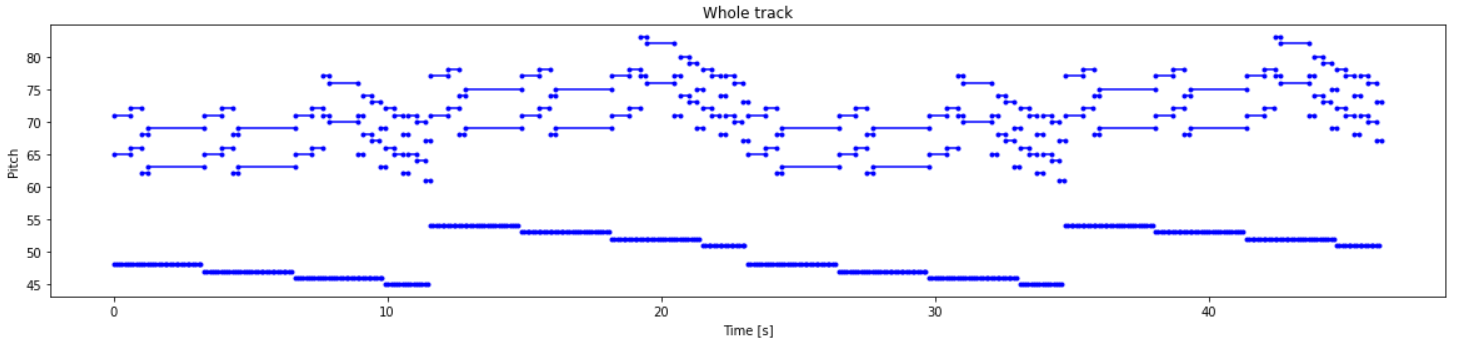
\includegraphics[width=0.5\textwidth]{./pics/fullSong.PNG}
\caption{Full Midi Sonng - "The Legend of Zelda - Death Mountain"}
\label{fig:fullSong}    
\end{figure}

All music files need to be read and changed by the program to acquire
a dataset for the neural network. A Long Short-Term Memory (LSTM) neural
network should be used to generate new melodies. A LSTM network is able to 
make predictions depending on a sequence of data. In terms of music this 
might mean that it can predict the next note by using a given sequence of 
multiple notes, that were played before.

With the help of the library "PrettyMidi" the Midi data is handled ~\cite{raffel_intuitive_2014-1}. All notes
from every Midi file is read and saved into an array. This array of tupels 
consists of the the pitch, the duration and the step of each note (step meaning
the length of the pause between the note and the note being played before).

Figure \ref{fig:verteilung} shows the distribution of pitch, step and duration
of all notes in the song "The Legend of Zelda - Death Mountain". The usage of 
low notes in contrast to really high notes is one of the key elements of 
the thrilling music of the Zelda games. Furthermore you can see, that the duration of
the notes are mostly short with only some outlier. 

\begin{figure}

\begin{minipage}{.5\linewidth}
\centering
\subfloat[]{\label{fig:test1}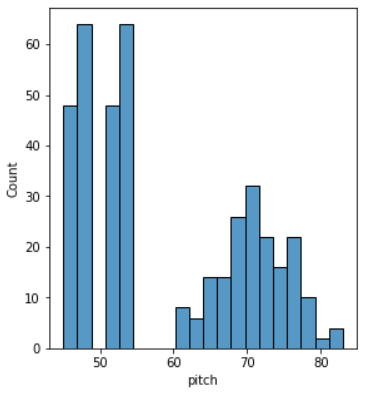
\includegraphics[scale=.5]{./pics/pitch.PNG}}
\end{minipage}%
\begin{minipage}{.5\linewidth}
\centering
\subfloat[]{\label{fig:test2}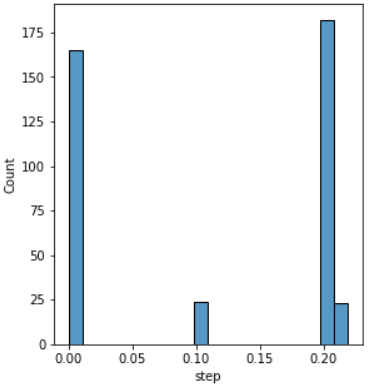
\includegraphics[scale=.5]{./pics/step.PNG}}
\end{minipage}\par
\centering
\subfloat[]{\label{fig:test3}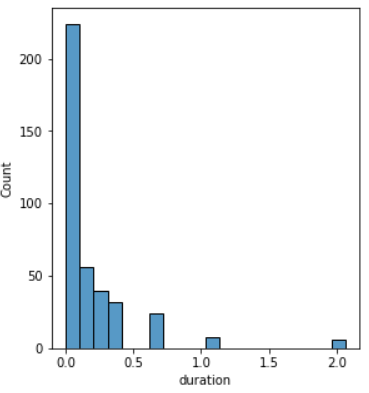
\includegraphics[scale=.5]{./pics/duration.PNG}}

\caption{Distribution of pitch, step and duration of "The Legend of Zelda - Death Mountain"}
\label{fig:verteilung}   
\end{figure}

So that the AI can be trained, the music data needs to be edited and sequences with a given 
length need to be created. A tensorflow dataset is created and filled with all notes (pitch, step and duration) ~\cite{noauthor_generate_nodate}.
To create sequences out of all the notes, the tensorflow dataset function "window" is used. It is used to 
create sequence windows of all available data and works by only seeing a window of data with given size, saving
it to a dataset of datasets and shifting the window to the next datapoint, creating a new window.
The sequence size is variable and dialed in at 50. This means, that a sequence consists of 50 notes and 
one result note as a label. The LSTM network learns what note should be played dependent on the 50 notes that were
played before.


After creating a dataset of datasets, it is necesarry to transform these into tensors, so that the network can
use them. The function "flat\_map" creates tensors from the dataset. The function to create sequences also normilizes 
the pitch of the notes to match the 128 possible pitches supported by "PrettyMidi". The new created tensorflow dataset
has a shape of (50, 3) meaning that the dataset has multiple sequences which consist of 50 notes each. The notes consist
of three parameters (pitch, duration and step).

The last part of preparing the dataset is to combine consecutive elements of the dataset into batches and to configure
the dataset for performance. First the current dataset is shuffled and then saved in batches. After that the function
"prefetch" is called on the dataset. It creates a new dataset that prefetches elements from this dataset. It allows later 
elements to be prepared while the current element is being processed ~\cite{noauthor_tfdatadataset_nodate}.

\section{Model}
\label{model}

After preparing the training dataset it is necessary to create and train the model. To create the model the now in tensorflow
embedded library "Keras" is used. The model will have one input layer with the shape of the created dataset. It also needs 
to have three outputs, one for each note variable.

A custom loss function for the step and the duration of the notes is needed. It is based on the mean squared error loss function
with positive pressure to ensure, that the model predicts mostly positive values for the step and duration. 

The complete model is shown in Figure \ref{fig:model}. It consists of an input layer with the input shape of the training data.
Furthermore it uses multiple LSTM layers that take a sequence as an input and can either return a sequence or a matrix. Dropout layers are
used to minimize overfitting the model because of the relativly small dataset used. Dropout layers randomly sets the input units to 0
at each step during training. This way the model will not be prone to overfitting. Dense layers are fully connected neural network
layers, where each input node is connected to each output node. Three dense layers are used as the output. The pitch output has 128 nodes 
which represent all the notes that can be used by "PrettyMidi". The duration and step layer only have one output node which
is a float value. This value should be positive and a custum loss function with positive pressure is needed to train
for those outputs (s. o.). The loss function "SparseCategoricalCrossentropy" is used for the pitch. The model is compiled with
an optimizer that implements the Adam algorithm and uses a learning rate of 0.0001.

The last LSTM layer isnt configured to return a sequence but a matrix. This way the output is flattened and dense layers can be connected.
The model has 2,793,602 configurable parameters and describes a rather small neural network.

\begin{figure}
\centering
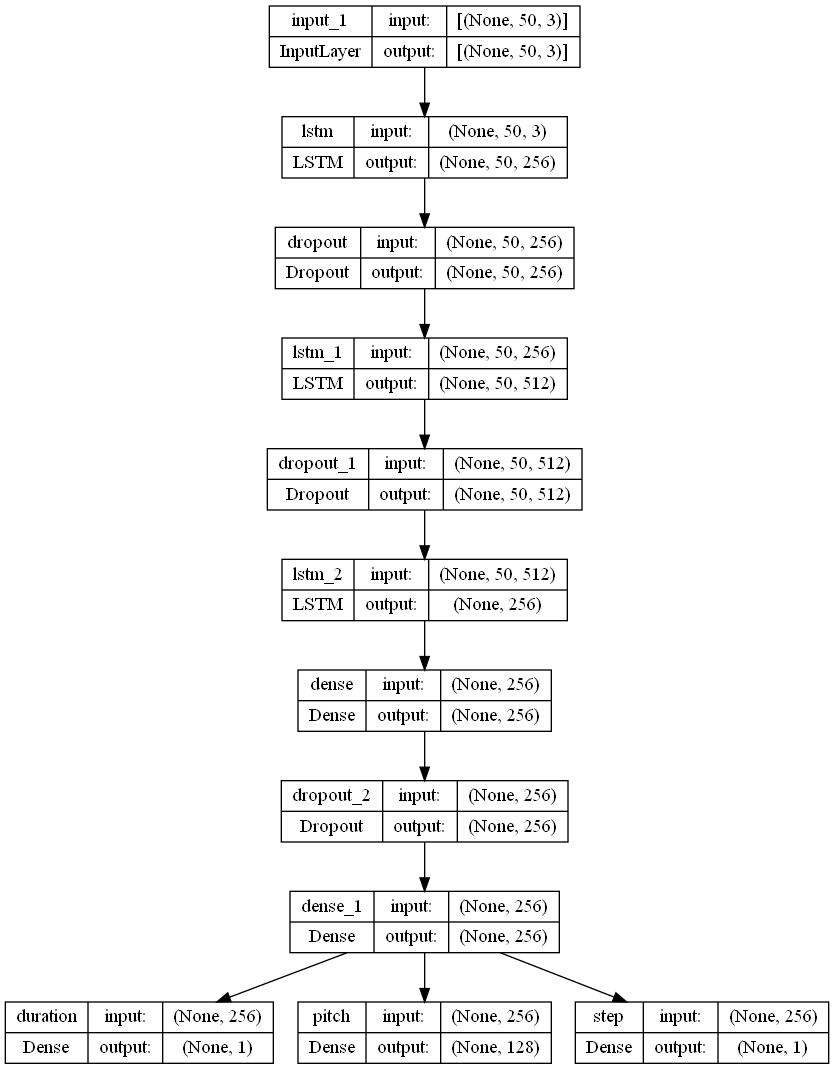
\includegraphics[width=0.5\textwidth]{./pics/model_plot.png}
\caption{Model}
\label{fig:model}    
\end{figure}

\section{Training}
\label{training}

After creating and compiling the model it is time to train it. First the starting loss values of each parameter is calculated. The following losses
are calculated:

\begin{itemize}
  \item loss: 5.442152976989746
  \begin{itemize}
  \item duration: 0.4956154227256775
  \item pitch: 4.851800918579102
  \item step: 0.094735287129879
  \end{itemize}
\end{itemize}

The pitch loss is sigificant greater then the loss of step and duration. The overall loss is calculated by adding all losses together.
To combat this, the model needs to be compiled with loss weights. The pitch loss is multiplied by 0.05 and the following losses 
are calculated:

\begin{itemize}
  \item loss: 0.8329412937164307
  \begin{itemize}
  \item duration: 0.4956154227256775
  \item pitch: 4.851800918579102
  \item step: 0.094735287129879
  \end{itemize}
\end{itemize}

Callback functions are used to create checkpoints of the model after each epoch it is running through. The weights from the model
are saved and the training can be halted and continued to not loose progress. Early stopping is also configured, to stop the 
training if multiple consecutive epochs do not lead to the reduction of the overall loss. This also helps if the loss suddenly
jumps to a higher value. Lowering the learning rate helped combat negative jumps of the overall loss.

After the configuration, the model is trained for a maximum of 500 epochs. Figure \ref{fig:loss} shows the progress of the 
overall loss over the generations. The training was halted after about 270 epochs because of no further change of the overall loss.
The training took about an hour of GPU processing time. The final overall loss is 0.0338.


\begin{figure}
\centering
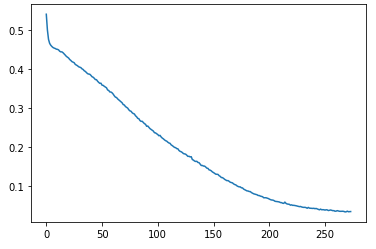
\includegraphics[width=0.5\textwidth]{./pics/Loss.PNG}
\caption{Added up loss over training generations}
\label{fig:loss}    
\end{figure}

\section{Music Generation}
\label{gen}

After training the model it is necessary to let notes be predicted by giving it a sequence of start notes. A function is 
written, that predicts the next note from a sequence of input notes. It uses the "predict" function of the tensorflow
model that was trained before. The function is implemented not to just pick the note pitch with the highest probability.
If the note with the highest probability would always be taken, the same input would generate the same next note. 
To still have variaty in the generation a temperature parameter is given into the function. This temperatur parameter is used
to create a small set of possible pitches for the next note. After that one of these notes gets randomly chosen.
The step and the duration have to be positive. If negative values are predicted the value gets set to zero.

To start the generation of multiple notes, a sequence of the trainingdata is used as an input to generate the next note.
A note will be generated and saved in an array of generated notes. The input sequence is altered by deleting the first
note and appending the new generated one. The next note is generated and also saved. After generating the given
amount of notes, the library "PrettyMidi" is used to create a Midi file out of the generated notes.

One possible output is shown in Figure \ref{fig:genNotes}. 


\begin{figure}
\centering
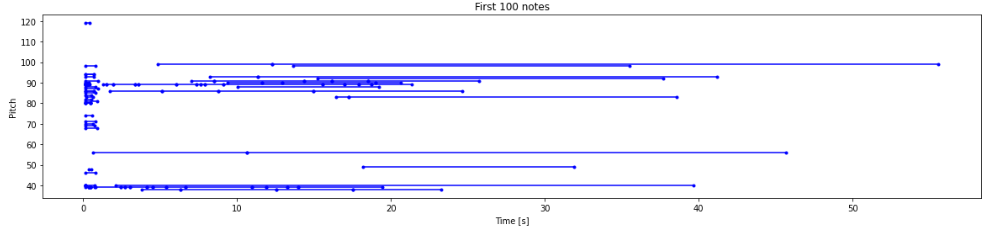
\includegraphics[width=0.5\textwidth]{./pics/genNotes.PNG}
\caption{Generated midi file}
\label{fig:genNotes}    
\end{figure}

\section{Results}
\label{res}

The generated notes in Figure \ref{fig:genNotes} look like random generated notes. At the beginning there is 
a cluster accord with a lot of short notes being played at the same time. A lot of the notes that were generated have 
a high duration. In Figure \ref{fig:genNotes} it is not possible to see all the short notes that make up most of
the song. Because of this, it is necessary to look at the distribution of all the notes of the song and compare these 
with the distribution from the training data. In Figure \ref{fig:verteilunggen} the distribution divided up in 
pitch, step and duration, is shown. 

In Figure \ref{fig:test11} you can see a seperation of the low and high notes just like in the distribution of the training
data. Zelda music (especially the battle music) uses the contrast of high and low notes to create tension. The step size and 
the duration of the notes are close to the training data aswell. This indicates that the model did learn how the music
of Zelda is composed and that it can predict notes that mimic this music.

\begin{figure}

\begin{minipage}{.5\linewidth}
\centering
\subfloat[]{\label{fig:test11}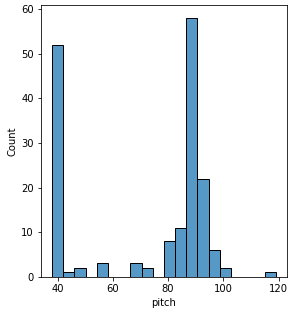
\includegraphics[scale=.5]{./pics/genPitch.PNG}}
\end{minipage}%
\begin{minipage}{.5\linewidth}
\centering
\subfloat[]{\label{fig:test21}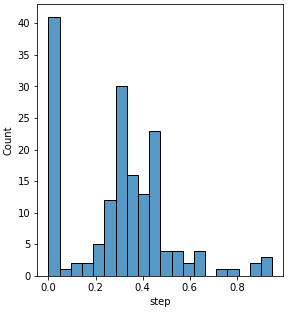
\includegraphics[scale=.5]{./pics/genStep.PNG}}
\end{minipage}\par
\centering
\subfloat[]{\label{fig:test31}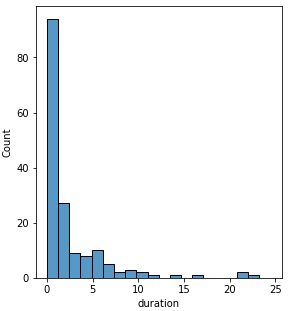
\includegraphics[scale=.5]{./pics/genDuration.PNG}}

\caption{Distribution of pitch, step and duration of generated music file}
\label{fig:verteilunggen}   
\end{figure}

\section{Conclusion}
\label{conc}

An LSTM neural network was trained with music of the popular videogame series Zelda.
65 Midi files from the videogame were used to train the model. Sequences of subsequent 
notes were created for training. The model was trained for about 270 epochs before the 
overall loss stagnated. By handing in a sequence of training data, it is possible to let
the model predict the next note. Multiple generated notes are saved in a Midi file.
The generated music does not sound great but the distribution of the generated notes
mirror the distribution of the training data.

In general the training of the model was a success even though the generated music is
not necessarily pleasant to the human ear. The generated music has similarities with
the training data, but also fluctuations of speed and additionally little harmony.
One reason could be the limited size of the dataset. With a bigger dataset the AI would
have been able to learn more and thus recreate the music with higher accuracy ~\cite{brownlee_impact_2019}.
The created dataset also consists of music for tense and calm scenarios in the gameplay.
The tense music is fast and has short notes that often alternate between high and low frequencies. 
Calm songs often consist of high melodies with longer notes. This mix of genres might also 
impair the generation of new notes.
As said before the generated music has little harmony. The current midi library is not able 
to detect accords in the file. Taking accords into account could improve the overall harmony
of the generated music. 

%\section{Section title}
%\label{sec:1}
%%Citations \cite{Ref1} and \cite{Ref2} and \cite{Ref3}.
%\subsection{Subsection title}
%\label{sec:2}
%as required. Don't forget to give each section
%and subsection a unique label (see Sect.~\ref{sec:1}).
%\paragraph{Paragraph headings} Use paragraph headings as needed.
%\begin{equation}
%a^2+b^2=c^2
%\end{equation}

% For one-column wide figures use
%\begin{figure}
%\centering
% Use the relevant command to insert your figure file.
% For example, with the graphicx package use
%  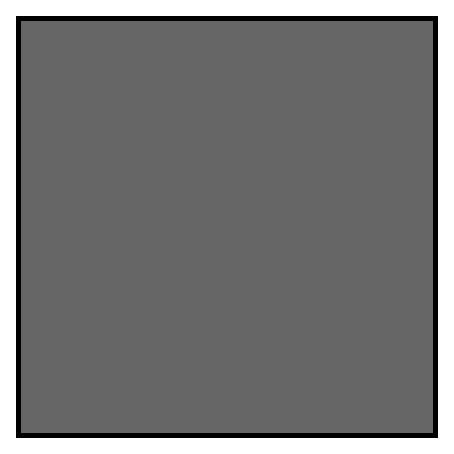
\includegraphics{example.eps}
% figure caption is below the figure
%\caption{Please write your figure caption here}
%\label{fig:1}       % Give a unique label
%\end{figure}
%
% For two-column wide figures use
%\begin{figure*}
%\centering
% Use the relevant command to insert your figure file.
% For example, with the graphicx package use
%  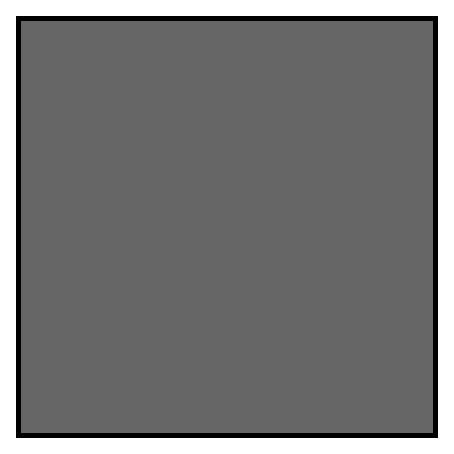
\includegraphics[width=0.75\textwidth]{example.eps}
% figure caption is below the figure
%\caption{Please write your figure caption here}
%\label{fig:2}       % Give a unique label
%\end{figure*}
%
% For tables use
%\begin{table}[t]
% table caption is above the table
%\caption{Please write your table caption here}
%\centering
%\label{tab:1}       % Give a unique label
% For LaTeX tables use
%\begin{tabular}{lll}
%\hline\noalign{\smallskip}
%first & second & third  \\[3pt]
%\tableheadseprule\noalign{\smallskip}
%number & number & number \\
%number & number & number \\
%\noalign{\smallskip}\hline
%\end{tabular}
%\end{table}


%\begin{acknowledgements}
%If you'd like to thank anyone, place your comments here
%and remove the percent signs.
%\end{acknowledgements}

% BibTeX users please use
\bibliographystyle{spmpsci}
\bibliography{zelda}   % name your BibTeX data base

% Non-BibTeX users please use
%\begin{thebibliography}{3}
%
% and use \bibitem to create references. Consult the Instructions
% for authors for reference list style.\cite{test:1}
%
% Format for Journal Reference
%\bibitem{Ref1}
%Author, I.: Article title. Journal Title-Abbreviated {\bf Vol}, pp--pp (year)
%% Format for books
%\bibitem{Ref2}
%Author, I., Smith, J.: Book Title. Publisher, Place (year)
% Format for proceedings
%\bibitem{Ref3}
%%Author, I., Smith, J.: Paper title. In: Editor, A. (ed.) Proceedings
%Title, Location, Date, pages. Publisher, Place (year)
% etc

%\end{thebibliography}

\begin{authorbiography}{example.eps}{Tim Luecking}\
Master student at the Bielefeld University of Applied Sciences, studying information technology.
\end{authorbiography}

\end{document}
% end of file template.tex
